\documentclass[twoside]{book}

% Packages required by doxygen
\usepackage{fixltx2e}
\usepackage{calc}
\usepackage{doxygen}
\usepackage[export]{adjustbox} % also loads graphicx
\usepackage{graphicx}
\usepackage[utf8]{inputenc}
\usepackage{makeidx}
\usepackage{multicol}
\usepackage{multirow}
\PassOptionsToPackage{warn}{textcomp}
\usepackage{textcomp}
\usepackage[nointegrals]{wasysym}
\usepackage[table]{xcolor}

% Font selection
\usepackage[T1]{fontenc}
\usepackage[scaled=.90]{helvet}
\usepackage{courier}
\usepackage{amssymb}
\usepackage{sectsty}
\renewcommand{\familydefault}{\sfdefault}
\allsectionsfont{%
  \fontseries{bc}\selectfont%
  \color{darkgray}%
}
\renewcommand{\DoxyLabelFont}{%
  \fontseries{bc}\selectfont%
  \color{darkgray}%
}
\newcommand{\+}{\discretionary{\mbox{\scriptsize$\hookleftarrow$}}{}{}}

% Page & text layout
\usepackage{geometry}
\geometry{%
  a4paper,%
  top=2.5cm,%
  bottom=2.5cm,%
  left=2.5cm,%
  right=2.5cm%
}
\tolerance=750
\hfuzz=15pt
\hbadness=750
\setlength{\emergencystretch}{15pt}
\setlength{\parindent}{0cm}
\setlength{\parskip}{3ex plus 2ex minus 2ex}
\makeatletter
\renewcommand{\paragraph}{%
  \@startsection{paragraph}{4}{0ex}{-1.0ex}{1.0ex}{%
    \normalfont\normalsize\bfseries\SS@parafont%
  }%
}
\renewcommand{\subparagraph}{%
  \@startsection{subparagraph}{5}{0ex}{-1.0ex}{1.0ex}{%
    \normalfont\normalsize\bfseries\SS@subparafont%
  }%
}
\makeatother

% Headers & footers
\usepackage{fancyhdr}
\pagestyle{fancyplain}
\fancyhead[LE]{\fancyplain{}{\bfseries\thepage}}
\fancyhead[CE]{\fancyplain{}{}}
\fancyhead[RE]{\fancyplain{}{\bfseries\leftmark}}
\fancyhead[LO]{\fancyplain{}{\bfseries\rightmark}}
\fancyhead[CO]{\fancyplain{}{}}
\fancyhead[RO]{\fancyplain{}{\bfseries\thepage}}
\fancyfoot[LE]{\fancyplain{}{}}
\fancyfoot[CE]{\fancyplain{}{}}
\fancyfoot[RE]{\fancyplain{}{\bfseries\scriptsize Generated by Doxygen }}
\fancyfoot[LO]{\fancyplain{}{\bfseries\scriptsize Generated by Doxygen }}
\fancyfoot[CO]{\fancyplain{}{}}
\fancyfoot[RO]{\fancyplain{}{}}
\renewcommand{\footrulewidth}{0.4pt}
\renewcommand{\chaptermark}[1]{%
  \markboth{#1}{}%
}
\renewcommand{\sectionmark}[1]{%
  \markright{\thesection\ #1}%
}

% Indices & bibliography
\usepackage{natbib}
\usepackage[titles]{tocloft}
\setcounter{tocdepth}{3}
\setcounter{secnumdepth}{5}
\makeindex

% Hyperlinks (required, but should be loaded last)
\usepackage{ifpdf}
\ifpdf
  \usepackage[pdftex,pagebackref=true]{hyperref}
\else
  \usepackage[ps2pdf,pagebackref=true]{hyperref}
\fi
\hypersetup{%
  colorlinks=true,%
  linkcolor=blue,%
  citecolor=blue,%
  unicode%
}

% Custom commands
\newcommand{\clearemptydoublepage}{%
  \newpage{\pagestyle{empty}\cleardoublepage}%
}

\usepackage{caption}
\captionsetup{labelsep=space,justification=centering,font={bf},singlelinecheck=off,skip=4pt,position=top}

%===== C O N T E N T S =====

\begin{document}

% Titlepage & ToC
\hypersetup{pageanchor=false,
             bookmarksnumbered=true,
             pdfencoding=unicode
            }
\pagenumbering{alph}
\begin{titlepage}
\vspace*{7cm}
\begin{center}%
{\Large My Project }\\
\vspace*{1cm}
{\large Generated by Doxygen 1.8.13}\\
\end{center}
\end{titlepage}
\clearemptydoublepage
\pagenumbering{roman}
\tableofcontents
\clearemptydoublepage
\pagenumbering{arabic}
\hypersetup{pageanchor=true}

%--- Begin generated contents ---
\chapter{Namespace Index}
\section{Packages}
Here are the packages with brief descriptions (if available)\+:\begin{DoxyCompactList}
\item\contentsline{section}{\hyperlink{namespace_biblioteka}{Biblioteka} }{\pageref{namespace_biblioteka}}{}
\item\contentsline{section}{\hyperlink{namespace_biblioteka_1_1_properties}{Biblioteka.\+Properties} }{\pageref{namespace_biblioteka_1_1_properties}}{}
\end{DoxyCompactList}

\chapter{Hierarchical Index}
\section{Class Hierarchy}
This inheritance list is sorted roughly, but not completely, alphabetically\+:\begin{DoxyCompactList}
\item Form\begin{DoxyCompactList}
\item \contentsline{section}{Biblioteka.\+About}{\pageref{class_biblioteka_1_1_about}}{}
\item \contentsline{section}{Biblioteka.\+authorization}{\pageref{class_biblioteka_1_1authorization}}{}
\item \contentsline{section}{Biblioteka.\+Form1}{\pageref{class_biblioteka_1_1_form1}}{}
\item \contentsline{section}{Biblioteka.\+Klient}{\pageref{class_biblioteka_1_1_klient}}{}
\item \contentsline{section}{Biblioteka.\+Książki}{\pageref{class_biblioteka_1_1_ksi_xC4_x85_xC5_xBCki}}{}
\item \contentsline{section}{Biblioteka.\+Pracownik}{\pageref{class_biblioteka_1_1_pracownik}}{}
\item \contentsline{section}{Biblioteka.\+Zamówienie}{\pageref{class_biblioteka_1_1_zam_xC3_xB3wienie}}{}
\end{DoxyCompactList}
\end{DoxyCompactList}

\chapter{Class Index}
\section{Class List}
Here are the classes, structs, unions and interfaces with brief descriptions\+:\begin{DoxyCompactList}
\item\contentsline{section}{\hyperlink{class_biblioteka_1_1_about}{Biblioteka.\+About} }{\pageref{class_biblioteka_1_1_about}}{}
\item\contentsline{section}{\hyperlink{class_biblioteka_1_1authorization}{Biblioteka.\+authorization} }{\pageref{class_biblioteka_1_1authorization}}{}
\item\contentsline{section}{\hyperlink{class_biblioteka_1_1_form1}{Biblioteka.\+Form1} }{\pageref{class_biblioteka_1_1_form1}}{}
\item\contentsline{section}{\hyperlink{class_biblioteka_1_1_klient}{Biblioteka.\+Klient} }{\pageref{class_biblioteka_1_1_klient}}{}
\item\contentsline{section}{\hyperlink{class_biblioteka_1_1_ksi_xC4_x85_xC5_xBCki}{Biblioteka.\+Książki} }{\pageref{class_biblioteka_1_1_ksi_xC4_x85_xC5_xBCki}}{}
\item\contentsline{section}{\hyperlink{class_biblioteka_1_1_pracownik}{Biblioteka.\+Pracownik} }{\pageref{class_biblioteka_1_1_pracownik}}{}
\item\contentsline{section}{\hyperlink{class_biblioteka_1_1_zam_xC3_xB3wienie}{Biblioteka.\+Zamówienie} }{\pageref{class_biblioteka_1_1_zam_xC3_xB3wienie}}{}
\end{DoxyCompactList}

\chapter{Namespace Documentation}
\hypertarget{namespace_biblioteka}{}\section{Biblioteka Namespace Reference}
\label{namespace_biblioteka}\index{Biblioteka@{Biblioteka}}
\subsection*{Namespaces}
\begin{DoxyCompactItemize}
\end{DoxyCompactItemize}
\subsection*{Classes}
\begin{DoxyCompactItemize}
\item 
class \hyperlink{class_biblioteka_1_1_about}{About}
\item 
class \hyperlink{class_biblioteka_1_1authorization}{authorization}
\item 
class \hyperlink{class_biblioteka_1_1_form1}{Form1}
\item 
class \hyperlink{class_biblioteka_1_1_klient}{Klient}
\item 
class \hyperlink{class_biblioteka_1_1_ksi_xC4_x85_xC5_xBCki}{Książki}
\item 
class \hyperlink{class_biblioteka_1_1_pracownik}{Pracownik}
\item 
class {\bfseries Program}
\item 
class \hyperlink{class_biblioteka_1_1_zam_xC3_xB3wienie}{Zamówienie}
\end{DoxyCompactItemize}

\hypertarget{namespace_biblioteka_1_1_properties}{}\section{Biblioteka.\+Properties Namespace Reference}
\label{namespace_biblioteka_1_1_properties}\index{Biblioteka.\+Properties@{Biblioteka.\+Properties}}
\subsection*{Classes}
\begin{DoxyCompactItemize}
\item 
class {\bfseries Resources}
\begin{DoxyCompactList}\small\item\em Класс ресурсов со строгим типом для поиска локализованных строк и пр. \end{DoxyCompactList}\item 
class {\bfseries Settings}
\end{DoxyCompactItemize}

\chapter{Class Documentation}
\hypertarget{class_biblioteka_1_1_about}{}\section{Biblioteka.\+About Class Reference}
\label{class_biblioteka_1_1_about}\index{Biblioteka.\+About@{Biblioteka.\+About}}
Inheritance diagram for Biblioteka.\+About\+:\begin{figure}[H]
\begin{center}
\leavevmode
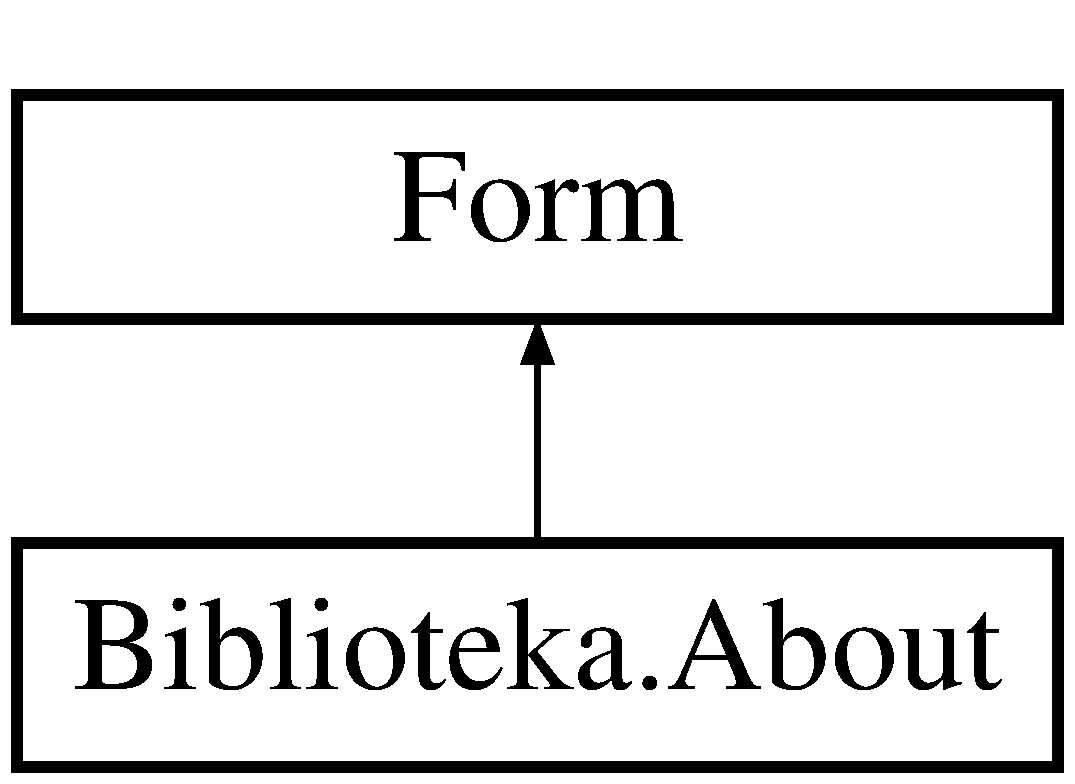
\includegraphics[height=2.000000cm]{class_biblioteka_1_1_about}
\end{center}
\end{figure}
\subsection*{Protected Member Functions}
\begin{DoxyCompactItemize}
\item 
override void \hyperlink{class_biblioteka_1_1_about_ae46b736c38521c1c20e00fad6979cdf9}{Dispose} (bool disposing)
\begin{DoxyCompactList}\small\item\em Clean up any resources being used. \end{DoxyCompactList}\end{DoxyCompactItemize}


\subsection{Member Function Documentation}
\mbox{\Hypertarget{class_biblioteka_1_1_about_ae46b736c38521c1c20e00fad6979cdf9}\label{class_biblioteka_1_1_about_ae46b736c38521c1c20e00fad6979cdf9}} 
\index{Biblioteka\+::\+About@{Biblioteka\+::\+About}!Dispose@{Dispose}}
\index{Dispose@{Dispose}!Biblioteka\+::\+About@{Biblioteka\+::\+About}}
\subsubsection{\texorpdfstring{Dispose()}{Dispose()}}
{\footnotesize\ttfamily override void Biblioteka.\+About.\+Dispose (\begin{DoxyParamCaption}\item[{bool}]{disposing }\end{DoxyParamCaption})\hspace{0.3cm}{\ttfamily [protected]}}



Clean up any resources being used. 


\begin{DoxyParams}{Parameters}
{\em disposing} & true if managed resources should be disposed; otherwise, false.\\
\hline
\end{DoxyParams}


The documentation for this class was generated from the following files\+:\begin{DoxyCompactItemize}
\item 
Biblioteka/About.\+cs\item 
Biblioteka/About.\+Designer.\+cs\end{DoxyCompactItemize}

\hypertarget{class_biblioteka_1_1authorization}{}\section{Biblioteka.\+authorization Class Reference}
\label{class_biblioteka_1_1authorization}\index{Biblioteka.\+authorization@{Biblioteka.\+authorization}}
Inheritance diagram for Biblioteka.\+authorization\+:\begin{figure}[H]
\begin{center}
\leavevmode
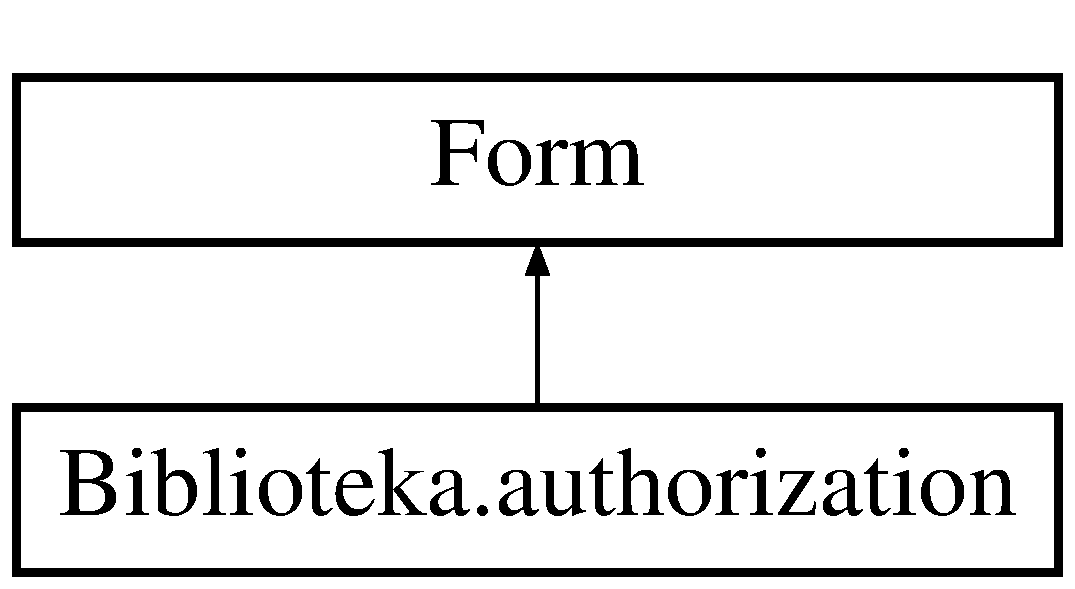
\includegraphics[height=2.000000cm]{class_biblioteka_1_1authorization}
\end{center}
\end{figure}
\subsection*{Protected Member Functions}
\begin{DoxyCompactItemize}
\item 
override void \hyperlink{class_biblioteka_1_1authorization_a93c2ea374a360b091974a617f76f63ac}{Dispose} (bool disposing)
\begin{DoxyCompactList}\small\item\em Clean up any resources being used. \end{DoxyCompactList}\end{DoxyCompactItemize}


\subsection{Member Function Documentation}
\mbox{\Hypertarget{class_biblioteka_1_1authorization_a93c2ea374a360b091974a617f76f63ac}\label{class_biblioteka_1_1authorization_a93c2ea374a360b091974a617f76f63ac}} 
\index{Biblioteka\+::authorization@{Biblioteka\+::authorization}!Dispose@{Dispose}}
\index{Dispose@{Dispose}!Biblioteka\+::authorization@{Biblioteka\+::authorization}}
\subsubsection{\texorpdfstring{Dispose()}{Dispose()}}
{\footnotesize\ttfamily override void Biblioteka.\+authorization.\+Dispose (\begin{DoxyParamCaption}\item[{bool}]{disposing }\end{DoxyParamCaption})\hspace{0.3cm}{\ttfamily [protected]}}



Clean up any resources being used. 


\begin{DoxyParams}{Parameters}
{\em disposing} & true if managed resources should be disposed; otherwise, false.\\
\hline
\end{DoxyParams}


The documentation for this class was generated from the following files\+:\begin{DoxyCompactItemize}
\item 
Biblioteka/authorization.\+cs\item 
Biblioteka/authorization.\+Designer.\+cs\end{DoxyCompactItemize}

\hypertarget{class_biblioteka_1_1_form1}{}\section{Biblioteka.\+Form1 Class Reference}
\label{class_biblioteka_1_1_form1}\index{Biblioteka.\+Form1@{Biblioteka.\+Form1}}
Inheritance diagram for Biblioteka.\+Form1\+:\begin{figure}[H]
\begin{center}
\leavevmode
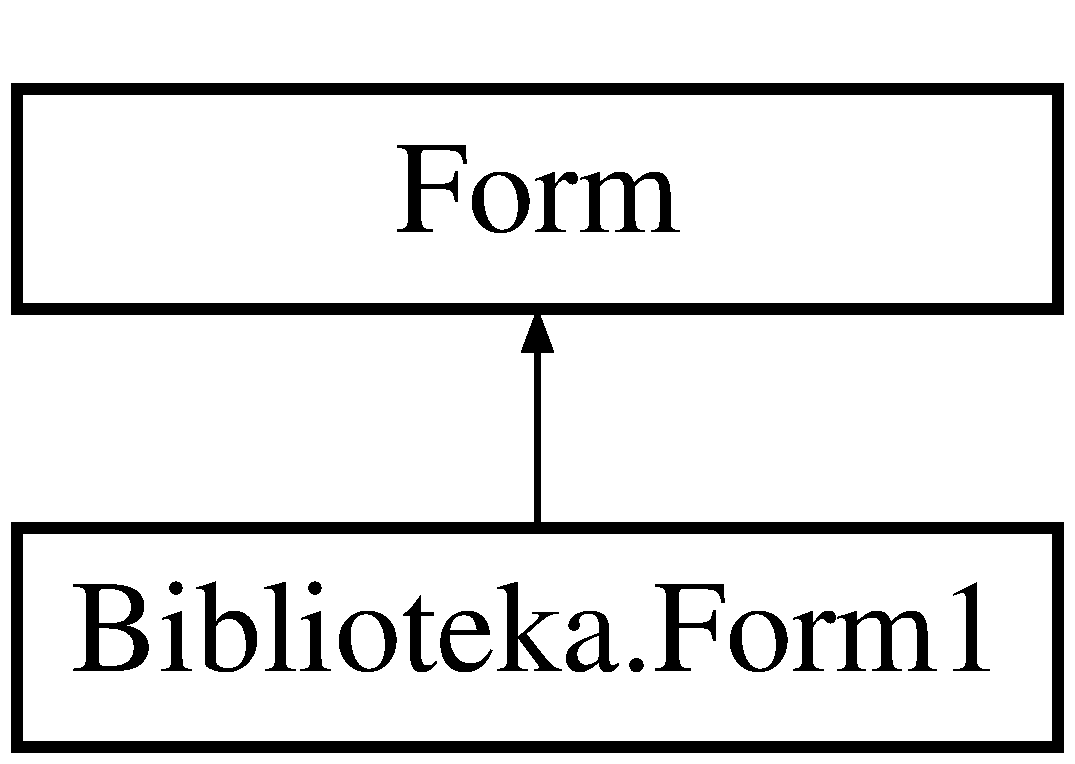
\includegraphics[height=2.000000cm]{class_biblioteka_1_1_form1}
\end{center}
\end{figure}
\subsection*{Protected Member Functions}
\begin{DoxyCompactItemize}
\item 
override void \hyperlink{class_biblioteka_1_1_form1_af5983327eaa75c22f4d1be3afd03b184}{Dispose} (bool disposing)
\begin{DoxyCompactList}\small\item\em Освободить все используемые ресурсы. \end{DoxyCompactList}\end{DoxyCompactItemize}


\subsection{Member Function Documentation}
\mbox{\Hypertarget{class_biblioteka_1_1_form1_af5983327eaa75c22f4d1be3afd03b184}\label{class_biblioteka_1_1_form1_af5983327eaa75c22f4d1be3afd03b184}} 
\index{Biblioteka\+::\+Form1@{Biblioteka\+::\+Form1}!Dispose@{Dispose}}
\index{Dispose@{Dispose}!Biblioteka\+::\+Form1@{Biblioteka\+::\+Form1}}
\subsubsection{\texorpdfstring{Dispose()}{Dispose()}}
{\footnotesize\ttfamily override void Biblioteka.\+Form1.\+Dispose (\begin{DoxyParamCaption}\item[{bool}]{disposing }\end{DoxyParamCaption})\hspace{0.3cm}{\ttfamily [protected]}}



Освободить все используемые ресурсы. 


\begin{DoxyParams}{Parameters}
{\em disposing} & истинно, если управляемый ресурс должен быть удален; иначе ложно.\\
\hline
\end{DoxyParams}


The documentation for this class was generated from the following files\+:\begin{DoxyCompactItemize}
\item 
Biblioteka/Form1.\+cs\item 
Biblioteka/Form1.\+Designer.\+cs\end{DoxyCompactItemize}

\hypertarget{class_biblioteka_1_1_klient}{}\section{Biblioteka.\+Klient Class Reference}
\label{class_biblioteka_1_1_klient}\index{Biblioteka.\+Klient@{Biblioteka.\+Klient}}
Inheritance diagram for Biblioteka.\+Klient\+:\begin{figure}[H]
\begin{center}
\leavevmode
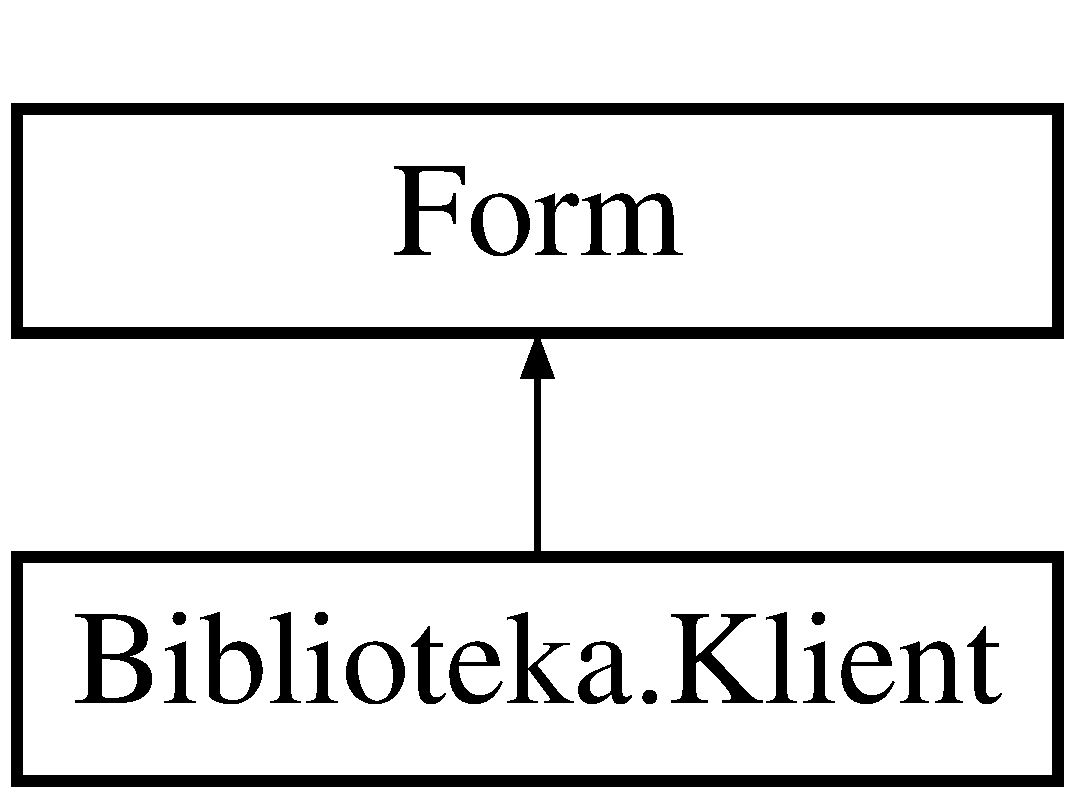
\includegraphics[height=2.000000cm]{class_biblioteka_1_1_klient}
\end{center}
\end{figure}
\subsection*{Protected Member Functions}
\begin{DoxyCompactItemize}
\item 
override void \hyperlink{class_biblioteka_1_1_klient_abc5ba28c26800c700600a2a19a1305f4}{Dispose} (bool disposing)
\begin{DoxyCompactList}\small\item\em Clean up any resources being used. \end{DoxyCompactList}\end{DoxyCompactItemize}


\subsection{Member Function Documentation}
\mbox{\Hypertarget{class_biblioteka_1_1_klient_abc5ba28c26800c700600a2a19a1305f4}\label{class_biblioteka_1_1_klient_abc5ba28c26800c700600a2a19a1305f4}} 
\index{Biblioteka\+::\+Klient@{Biblioteka\+::\+Klient}!Dispose@{Dispose}}
\index{Dispose@{Dispose}!Biblioteka\+::\+Klient@{Biblioteka\+::\+Klient}}
\subsubsection{\texorpdfstring{Dispose()}{Dispose()}}
{\footnotesize\ttfamily override void Biblioteka.\+Klient.\+Dispose (\begin{DoxyParamCaption}\item[{bool}]{disposing }\end{DoxyParamCaption})\hspace{0.3cm}{\ttfamily [protected]}}



Clean up any resources being used. 


\begin{DoxyParams}{Parameters}
{\em disposing} & true if managed resources should be disposed; otherwise, false.\\
\hline
\end{DoxyParams}


The documentation for this class was generated from the following files\+:\begin{DoxyCompactItemize}
\item 
Biblioteka/Klient.\+cs\item 
Biblioteka/Klient.\+Designer.\+cs\end{DoxyCompactItemize}

\hypertarget{class_biblioteka_1_1_ksi_xC4_x85_xC5_xBCki}{}\section{Biblioteka.\+Książki Class Reference}
\label{class_biblioteka_1_1_ksi_xC4_x85_xC5_xBCki}\index{Biblioteka.\+Książki@{Biblioteka.\+Książki}}
Inheritance diagram for Biblioteka.\+Książki\+:\begin{figure}[H]
\begin{center}
\leavevmode
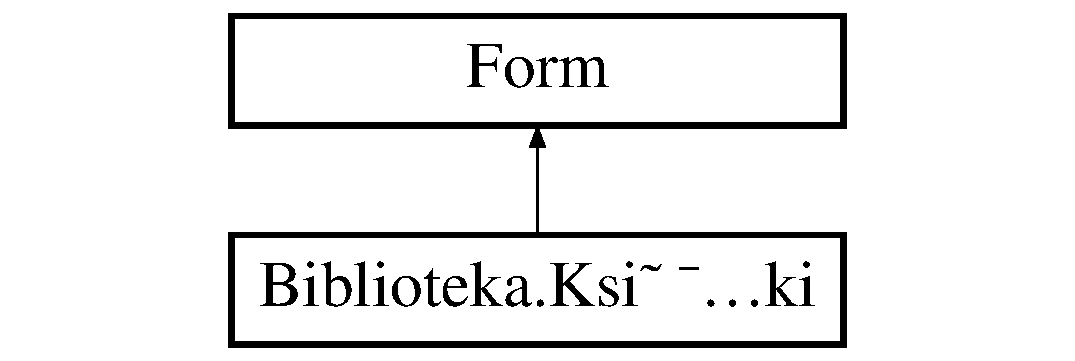
\includegraphics[height=2.000000cm]{class_biblioteka_1_1_ksi_xC4_x85_xC5_xBCki}
\end{center}
\end{figure}
\subsection*{Protected Member Functions}
\begin{DoxyCompactItemize}
\item 
override void \hyperlink{class_biblioteka_1_1_ksi_xC4_x85_xC5_xBCki_a3b820e000ec4ac60b7dc5d7c9da7660b}{Dispose} (bool disposing)
\begin{DoxyCompactList}\small\item\em Clean up any resources being used. \end{DoxyCompactList}\end{DoxyCompactItemize}


\subsection{Member Function Documentation}
\mbox{\Hypertarget{class_biblioteka_1_1_ksi_xC4_x85_xC5_xBCki_a3b820e000ec4ac60b7dc5d7c9da7660b}\label{class_biblioteka_1_1_ksi_xC4_x85_xC5_xBCki_a3b820e000ec4ac60b7dc5d7c9da7660b}} 
\index{Biblioteka\+::\+Książki@{Biblioteka\+::\+Książki}!Dispose@{Dispose}}
\index{Dispose@{Dispose}!Biblioteka\+::\+Książki@{Biblioteka\+::\+Książki}}
\subsubsection{\texorpdfstring{Dispose()}{Dispose()}}
{\footnotesize\ttfamily override void Biblioteka.\+Książki.\+Dispose (\begin{DoxyParamCaption}\item[{bool}]{disposing }\end{DoxyParamCaption})\hspace{0.3cm}{\ttfamily [protected]}}



Clean up any resources being used. 


\begin{DoxyParams}{Parameters}
{\em disposing} & true if managed resources should be disposed; otherwise, false.\\
\hline
\end{DoxyParams}


The documentation for this class was generated from the following files\+:\begin{DoxyCompactItemize}
\item 
Biblioteka/Książki.\+cs\item 
Biblioteka/Książki.\+Designer.\+cs\end{DoxyCompactItemize}

\hypertarget{class_biblioteka_1_1_pracownik}{}\section{Biblioteka.\+Pracownik Class Reference}
\label{class_biblioteka_1_1_pracownik}\index{Biblioteka.\+Pracownik@{Biblioteka.\+Pracownik}}
Inheritance diagram for Biblioteka.\+Pracownik\+:\begin{figure}[H]
\begin{center}
\leavevmode
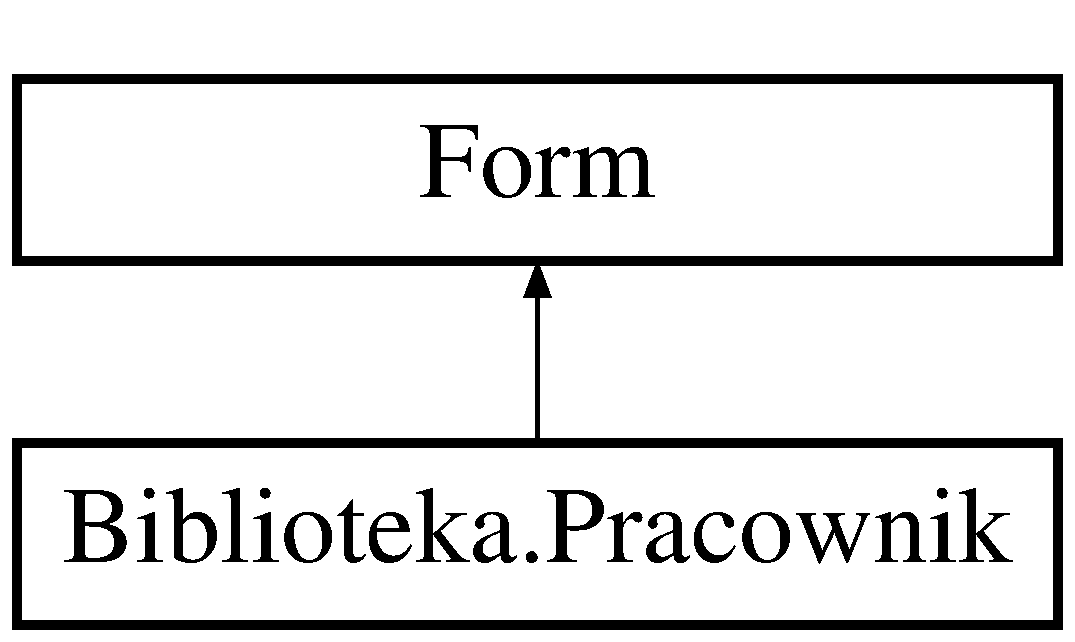
\includegraphics[height=2.000000cm]{class_biblioteka_1_1_pracownik}
\end{center}
\end{figure}
\subsection*{Protected Member Functions}
\begin{DoxyCompactItemize}
\item 
override void \hyperlink{class_biblioteka_1_1_pracownik_a62a6ef549abc407e62d0992080bd8709}{Dispose} (bool disposing)
\begin{DoxyCompactList}\small\item\em Clean up any resources being used. \end{DoxyCompactList}\end{DoxyCompactItemize}


\subsection{Member Function Documentation}
\mbox{\Hypertarget{class_biblioteka_1_1_pracownik_a62a6ef549abc407e62d0992080bd8709}\label{class_biblioteka_1_1_pracownik_a62a6ef549abc407e62d0992080bd8709}} 
\index{Biblioteka\+::\+Pracownik@{Biblioteka\+::\+Pracownik}!Dispose@{Dispose}}
\index{Dispose@{Dispose}!Biblioteka\+::\+Pracownik@{Biblioteka\+::\+Pracownik}}
\subsubsection{\texorpdfstring{Dispose()}{Dispose()}}
{\footnotesize\ttfamily override void Biblioteka.\+Pracownik.\+Dispose (\begin{DoxyParamCaption}\item[{bool}]{disposing }\end{DoxyParamCaption})\hspace{0.3cm}{\ttfamily [protected]}}



Clean up any resources being used. 


\begin{DoxyParams}{Parameters}
{\em disposing} & true if managed resources should be disposed; otherwise, false.\\
\hline
\end{DoxyParams}


The documentation for this class was generated from the following files\+:\begin{DoxyCompactItemize}
\item 
Biblioteka/Pracownik.\+cs\item 
Biblioteka/Pracownik.\+Designer.\+cs\end{DoxyCompactItemize}

\hypertarget{class_biblioteka_1_1_zam_xC3_xB3wienie}{}\section{Biblioteka.\+Zamówienie Class Reference}
\label{class_biblioteka_1_1_zam_xC3_xB3wienie}\index{Biblioteka.\+Zamówienie@{Biblioteka.\+Zamówienie}}
Inheritance diagram for Biblioteka.\+Zamówienie\+:\begin{figure}[H]
\begin{center}
\leavevmode
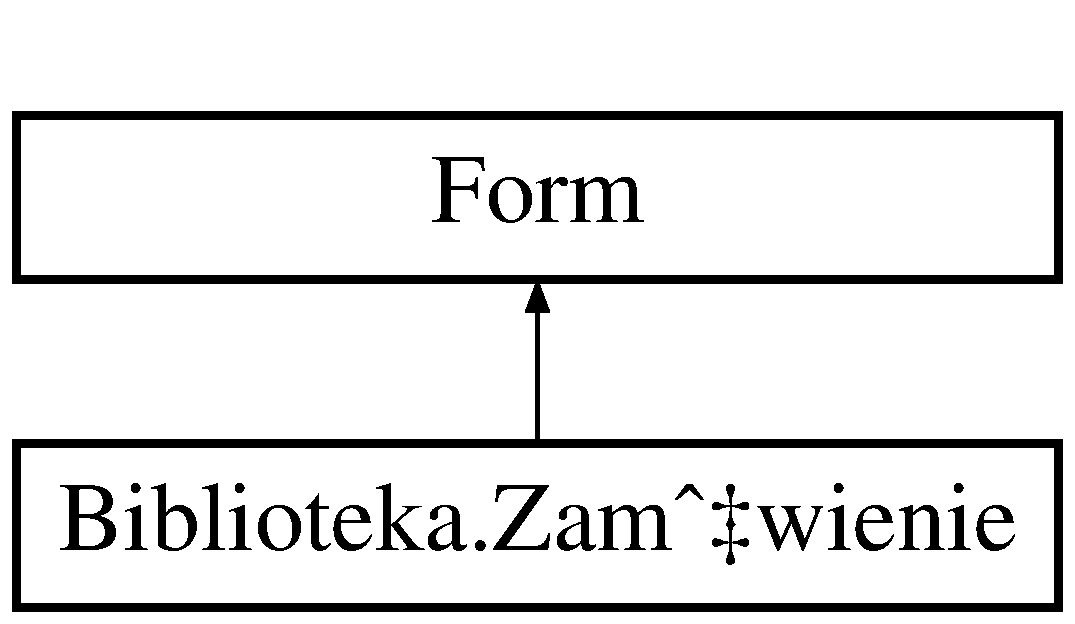
\includegraphics[height=2.000000cm]{class_biblioteka_1_1_zam_xC3_xB3wienie}
\end{center}
\end{figure}
\subsection*{Protected Member Functions}
\begin{DoxyCompactItemize}
\item 
override void \hyperlink{class_biblioteka_1_1_zam_xC3_xB3wienie_a1398f1e24c48fa539f5afe91527eec6f}{Dispose} (bool disposing)
\begin{DoxyCompactList}\small\item\em Clean up any resources being used. \end{DoxyCompactList}\end{DoxyCompactItemize}


\subsection{Member Function Documentation}
\mbox{\Hypertarget{class_biblioteka_1_1_zam_xC3_xB3wienie_a1398f1e24c48fa539f5afe91527eec6f}\label{class_biblioteka_1_1_zam_xC3_xB3wienie_a1398f1e24c48fa539f5afe91527eec6f}} 
\index{Biblioteka\+::\+Zamówienie@{Biblioteka\+::\+Zamówienie}!Dispose@{Dispose}}
\index{Dispose@{Dispose}!Biblioteka\+::\+Zamówienie@{Biblioteka\+::\+Zamówienie}}
\subsubsection{\texorpdfstring{Dispose()}{Dispose()}}
{\footnotesize\ttfamily override void Biblioteka.\+Zamówienie.\+Dispose (\begin{DoxyParamCaption}\item[{bool}]{disposing }\end{DoxyParamCaption})\hspace{0.3cm}{\ttfamily [protected]}}



Clean up any resources being used. 


\begin{DoxyParams}{Parameters}
{\em disposing} & true if managed resources should be disposed; otherwise, false.\\
\hline
\end{DoxyParams}


The documentation for this class was generated from the following files\+:\begin{DoxyCompactItemize}
\item 
Biblioteka/Zamówienie.\+cs\item 
Biblioteka/Zamówienie.\+Designer.\+cs\end{DoxyCompactItemize}

%--- End generated contents ---

% Index
\backmatter
\newpage
\phantomsection
\clearemptydoublepage
\addcontentsline{toc}{chapter}{Index}
\printindex

\end{document}
